\section{Development Methodology}\label{Development Methodology} 
    We did not follow any established development methodology, such as \gls{scrum}\footnote{\gls{scrum} - An agile software development methodology. [\url{http://en.wikipedia.org/wiki/Scrum_(development)}]} or \gls{xp}\footnote{\gls{xp} - A type of agile software development. [\url{http://en.wikipedia.org/wiki/Extreme_programming_practices}]}, as this project required more planning and configuration of existing solutions, than actual coding. In the process of choosing a development methodology we considered scrum, waterfall, agile, xp, and some others in addition to combination of these. In the end we chose a mix of the \gls{waterfall}\footnote{\gls{waterfall} - A sequential design process. [\url{http://en.wikipedia.org/wiki/Waterfall_development}]} and \gls{agile}\footnote{\gls{agile} - A group of software development methodologies based on iterative and incremental development. [\url{http://en.wikipedia.org/wiki/Agile_software_development}]}, we discuss these decisions in the sections below. You will also find a list of the tools we chose to work with, and why we decided to use them. 
    
    Because this is a research project, the customer will act more as an advisor than a customer, and will have more suggestions and advice than demands and requirements. We have been given a clear understanding of what the final product should be, and we have a list of requirements that should be met. Other than that, we are relatively free regarding how we go about solving the problem. Because of this, a single methodology, like Scrum, won't work for us, as it requires us to be in close and frequent contact with the customer, presenting a prototype every other week and continue development based on the customers feedback and demands.
    
    As mentioned, this is a project that requires quite a lot of planning before any programming can be done. This necessitates that we start the development according to a waterfall model in terms of the architecture planning as well as the requirements specification. By using the waterfall model in these first phases, we ensure that the plannning is done thoroughly to minimize the ammount of trial and error during the later implementation phase.
    
    As the project progresses we’ll be switching to a more agile development method, in order to allow iterative development and facilitate any necessary changes that may turn up as code is produced, as opposed to waterfall-coding, where we have to strictly follow our plans. Agile also lets us use the flat organisational structure we have chosen, which we believe will greatly help cooperation within the team.
    
    % TODO: 
    %compare scrum/agile and waterfall, to see why waterfall is better for our project. 
    %describe what we actually did use in the end. 
    

    \subsection{Project Organization}\label{Project Organization}
    
    We have devided the project tasks in to work packages. These packages are represented in a \gls{wbs}\footnote{\gls{wbs} - An oriented decomposition of a project into smaller components. [\url{http://en.wikipedia.org/wiki/Work_breakdown_structure}]} (\ref{Work Breakdown Structure}). The schedule for the project is represented in a \gls{gantt}\footnote{\gls{gantt} - A type of bar chart that illustrates a project schedule. [\url{http://en.wikipedia.org/wiki/Gantt}]} (Fig.\ref{fig:gantt}). The figure is part of our full Gantt chart. As the full diagram cannot be included nicely in the report we have attached it as an HTML document (\ref{File Attachments}).
     
        \begin{figure}[h]
            \centering
            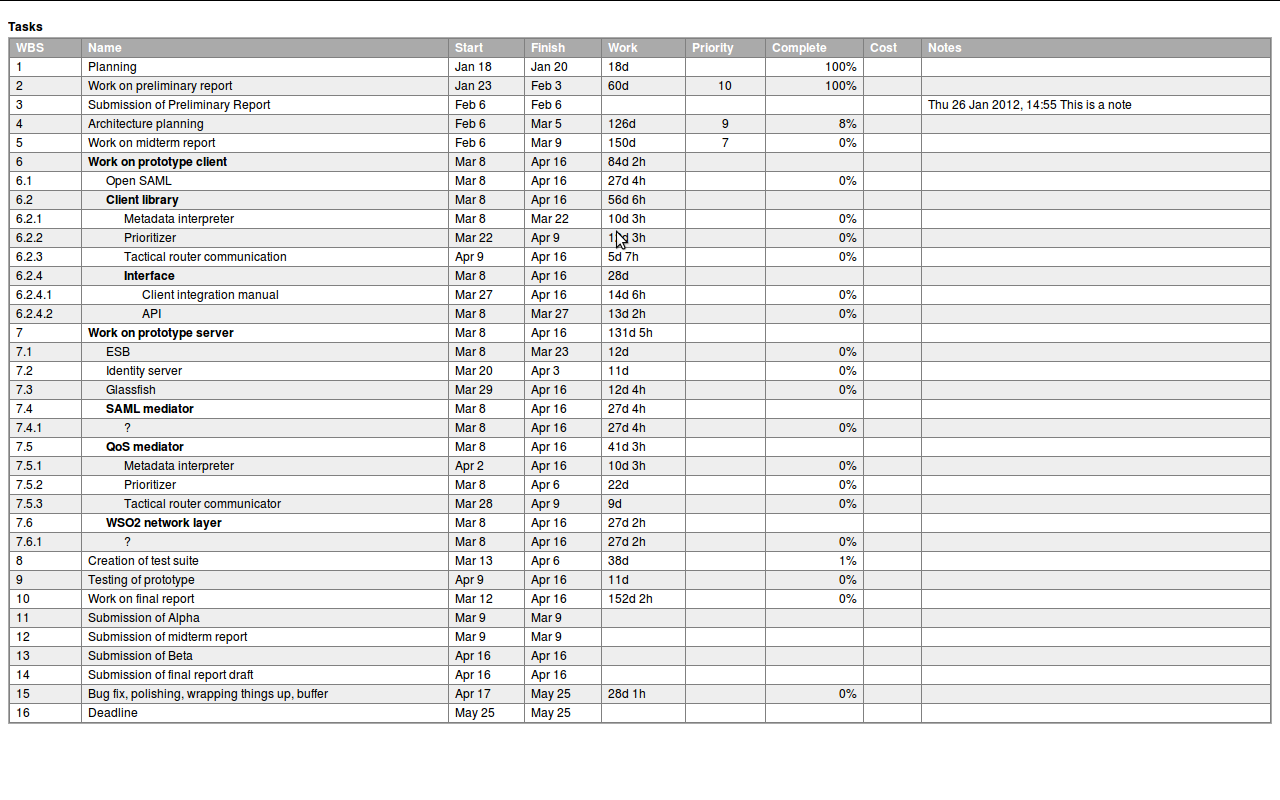
\includegraphics[width=\textwidth]{gantt}
            \caption{Part of our Gantt diagram} 
            This is an example to show that the gantt diagram exists and what it looks like. Se full diagram in attachments: (\ref{File Attachments})
            \label{fig:gantt}
        \end{figure}
    
    
    \subsection{Software project life cycle}\label{Software project life cycle}
    
    For our project life cycle we chose agile. Originally we started out with the intention of using Scrum and Scrum only. That idea was quickly scrapped as we found out that our task was very research heavy. This made us rethink our approach to the development cycle and turn in the direction of agile software development.
    
    %What mede us think scrum was usefull in the beginning. 
    Early in the project we expected that we could begin coding and prototyping before too long. This proved to be wrong as there was a lot of research to be done. Scrum was originally a tactic to improve product flexibility and production speed. This works very well in software development when you already know what you are supposed to do and the major part of the task is to implement the required functionality. When the functionality has to be designed and researched extensively, scrum becomes unsuitable. 
    
    With the agile method there is elements that suits us better then others. "Individuals and Interaction" and "Customer Collaboration" are two important elements that we use. The full description of the agile method can be found in the Agile Manifesto\footnote
        {Agile Manifesto, the key elements of the agile software development method. [\href{http://http://agilemanifesto.org/}{AgileManifesto.org}]}.
    
    %elaborate the benefits and usage of individuals and interaction
    Individuals and interactions are strongly connected with the organization of our team (\ref{Team Organization}). The flat team structure force us to have a good dialog among the group members. This increase the team members interaction and strengthens the team communication. The strengthened communication promotes the individuals of the group and the team members confidence, which in turn increases the total productivity of the group. The frequent interactions with the customer are also a part of our adaption to the agile development method. 
    
    %elaborate the benefits and usage of Customer collaboration.
    Customer Collaboration is the aspect of the group contacting the customer and keeping a good dialog with them. This is to make sure that we produce a product that the customer wants. To achieve this part of the agile manifesto we have meetings with the customer every week and have frequent email correspondence to iron out the bumps of our product. The frequent communication with the customer helps us to create a more precise and consistent system with better documentation. The main part of the communication with the customer is for the benefit of the project and constant improvement. The constant improvement and iterative work flow is a central part of the agile method. 

    % TODO: write a comparriosom of scrum ws waterfall. 
    Waterfall vs Scrum, to be continued. 

    \subsection{System Technology}\label{System Technology}
    
    We  intend to do a test driven development in order to achieve high quality code. This will give us something to test while we are working, and it will also give us a great way to tell if some new piece of code gets in the way of previously written code. For this purpose we will use \gls{junit}\footnote{\gls{junit} - A testing framework for the Java programming language. [\url{http://junit.org/}]} as the testing framework. We will also be doing periodical code reviews approximately every two weeks of development, synchronized with a code/feature freeze where we make sure everything works. As the customer wanted extensive testing of the middleware, we agreed to do testing on the network emulator NS3, as we have someone in the group already familiar with it. The advantage of using NS3 will be extensive testing, but also a great deal of empirical and verifiable data, which the customer can also use to evaluate the product.

    We will use \gls{git}\footnote{\gls{git} - A free and open source, distributed version control system. [\url{http://www.git-scm.com}]} and \gls{github}\footnote{\gls{github} - A web-based hosting service for software development projects that use the Git version control system. [\url{http://www.github.com}]} to handle our file repository, although Google Docs will be used for easy sharing and collaboration of schedules, meeting minutes, and reports. Even though the course set us up to use \gls{svn} (SVN)\footnote{\gls{svn} - A version control system}, we decided against this as Git gives us more options to develop code which will not greatly affect other parts of the code base before we decide to integrate it. To this extent we have decided that we should take advantage of Git’s built in support for ‘branches’ as much as possible. The argument for using Google Docs is that we have the possibility of editing a document together and easy sharing of documents. Delivered reports will be created with \gls{latex}\footnote{\gls{latex} - A document preparation system for the \TeX -typesetting program}, which we prefer over standard word processors. Our GitHub repository is open to the public, and the software will be released as open source, most likely under the Apache License.\footnote{\url{http://www.apache.org/licenses/LICENSE-2.0.html}} In some places we are forced to use the ASF, like the changes we have done to Apache HTTPComponents and Apache Synapse, but as the licenses allows for derived works to be licensed under a different license we are free to chose a different one. The Apache License version 2.0 is also compatible with the GPLv3 so there is no problem for us in using either. 
    We argreed to use the Apache2 license. FFI could not find any negativities for them in the license so we decided to use it. 

    Each of us is free to choose his own \gls{ide}\footnote{\gls{ide} - Integrated Development Environment} for programming. Because we are using Git, there should be no problem in using the IDE of our choice, and this gives us the added advantage that each person can use the tool which he is most comfortable with. We will stick to the standard \gls{java coding conventions}.
    
    Since we were so free to choose which tools we wanted to use we decided that this list should be quite lightweight. However the list compiled should be an indication of what is needed for the project. Some of the tools were chosen by us as is and other were demanded by needs of other components. All tools used can be  upgraded, downgraded or dropped during the course of this project. The final report will contain the official list as such this list is not in any way final. Our final report will also contain a list with supported tools tested with the final product.
    \begin{itemize}
    % TODO: we must have a full list of tested versions of technologies in the full version of this report, probably under testing.
        \item Git version 1.7.x
        \item Java version 1.6.x
        \item Free choice of IDE
        \item JUnit version 4.x
        \item NS3 version 3.13
        \item WSO2 ESB 4.0.3
        \item Axiom version 1.2.11  -  Note that our server code must use the same version of axiom as the ESB.
	\item HTTPCore version 4.1.4
	\item Commons-logging version 1.1.1
	\item MobiEmu
    \end{itemize}
    

